\usetikzlibrary{calc,arrows.meta,positioning,backgrounds}
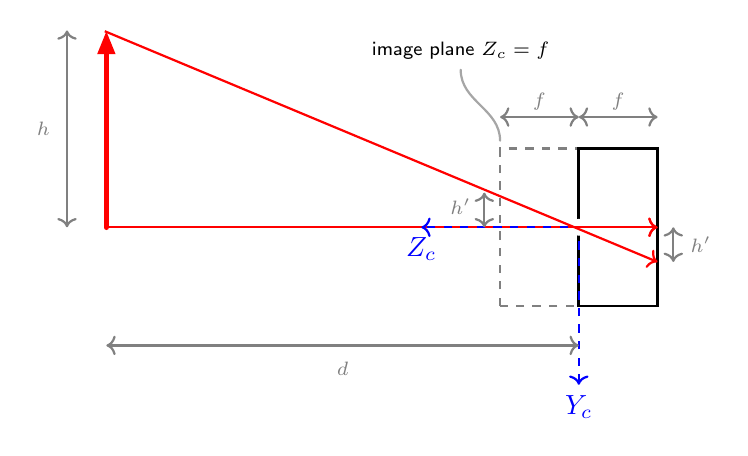
\begin{tikzpicture} [
    description/.style={draw=gray!70, thick, line cap=round, every node/.style={align=center, font=\scriptsize\sffamily, anchor=north}},
	imagearrow/.style={red, line cap=round, -{Triangle[width=3*#1]}, line width=#1, shorten >=#1*0*1.75pt, every node/.append style={fill, circle, inner sep=0pt, minimum size=#1*3.5pt, anchor=center, outer sep=0pt}}
  ]

\definecolor{mygreen}{RGB}{28, 150, 28}

%boxes
\draw[gray,line width=1, dashed] (6,-1) rectangle (7,1);
\draw[line width=1] (7,-1) rectangle (8,1);

% object 
\draw[imagearrow=2] (1,0) -- (1,2.5);


%light ray from bottom
\draw[red, ->, thick] (1,0) -- (8,0);

% coordinate systems
\draw [<->,thick, blue, dashed] (7,-2) node (yaxis) [below] {$Y_c$}
        |- (5,0) node (xaxis) [below] {$Z_c$};


% pinhole
\draw[color=white, fill] (7,0) circle (0.1);
% redraw part of red light ray that was deleted (hacky!)
\draw[red, ->, thick] (6.88,0) -- (8,0);

% light ray from top
\draw[red, ->, thick] (0.98,2.49) -- (8,-0.44);


% descriptions
%\path[description](1,2.6) [out=90, in=270] to (2,3) node[above] {Point $P$ \\ $(X_c=0,Y_c=-h,Z_c=d)$};
%\path[description](8.1,-0.44) [out=0, in=90] to (10,-2) node[below] {image of $P$ \\$(X_c=0,Y_c=h',Z_c=-f)$};
%\path[description](5.94,0.48) [out=90+45, in=270] to (7,3) node[above] {virtual image of $P$ \\$(X_c=0,Y_c=h',Z_c=f)$};
\path[description](6,1.1) [out=90, in=-90] to (5.5,2) node[above] {image plane $Z_c=f$};


%length

\draw[gray, <->, thick] (7,1.4) -- (8,1.4);
\draw[gray] (7.5,1.6) node{\scriptsize $f$};

\draw[gray, <->, thick] (6,1.4) -- (7,1.4);
\draw[gray] (6.5,1.6) node{\scriptsize $f$};

\draw[gray, <->, thick] (8.2,-0.44) -- (8.2,0);
\draw[gray] (8.55,-0.22) node{\scriptsize $h'$};

\draw[gray, <->, thick] (5.8,0.44) -- (5.8,0);
\draw[gray] (5.5,0.26) node{\scriptsize $h'$};

\draw[gray, <->, thick] (0.5,0) -- (0.5,2.5);
\draw[gray] (0.2,1.25) node{\scriptsize $h$};

\draw[gray, <->, thick] (1,-1.5) -- (7,-1.5);
\draw[gray] (4,-1.8) node{\scriptsize $d$};

\end{tikzpicture}